\documentclass{article}
\usepackage[paperheight=8.5in,paperwidth=5.5in,margin=0in]{geometry}
\usepackage{tikz}
\usetikzlibrary{shadings,patterns,fadings}
\usepackage{chancery}

\def\titre{titreARemplacer}

\begin{document}
\begin{tikzpicture}[remember picture, overlay]
    % Image de fond
    \node[anchor=center, opacity=0.6] at (current page.center) {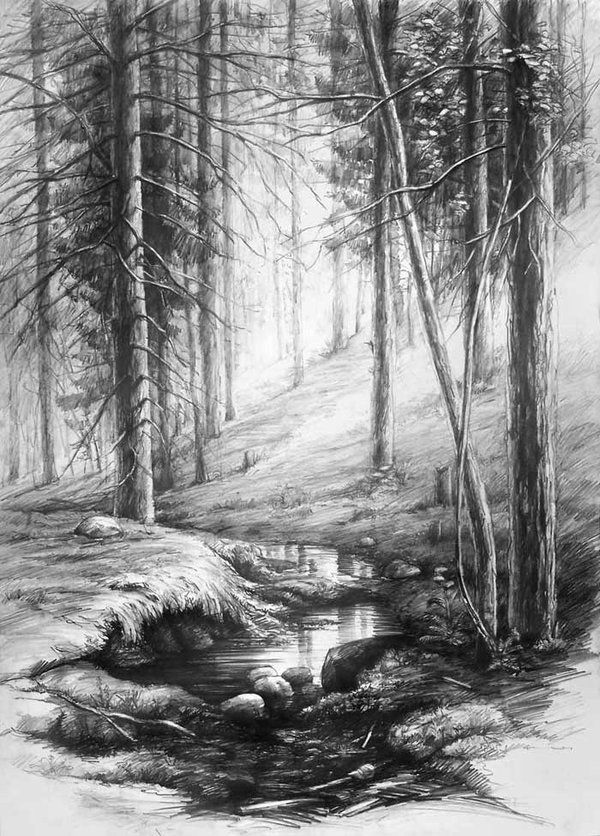
\includegraphics[width=\paperwidth,height=\paperheight]{imageCouverture}};
    
    \foreach \i in {0,...,250} {
    % Calcul de l'opacité avec une courbe en cloche
    \pgfmathsetmacro{\opacity}{0.3 * exp(-pow((\i-125)/25,2))}
    % Calcul de la position verticale (déplacée de 2 unités vers le bas)
    \pgfmathsetmacro{\ypos}{-3.1 - (\i * 3/250)} % -4 au lieu de -2
    % Dessiner le rectangle avec l'opacité calculée
    \fill[white, opacity=\opacity] (-1,\ypos) rectangle (13.5,{-3.1 - ((\i+1) * 2/250)}); % -4 au lieu de -2
    }
    %\fill[white] (-1,-4.1) rectangle (14,-4.6); 
        % Titre
    \node[anchor=center, minimum height=2cm, minimum width=13.9cm, font=\LARGE, text=gray!95] at (6.45,-4.4) {\textsw{\titre}};

    %WEIRD AUSSI
    % \foreach \i in {0,...,500} {
    %     % Calcul de l'opacité avec une courbe en cloche
    %     \pgfmathsetmacro{\opacity}{0.045 * exp(-pow((\i-250)/50,2))}
    %     \pgfmathsetmacro{\ypos}{-2 - (\i * 6/500)}
    %     \fill[white, opacity=\opacity] (-1,\ypos) rectangle (13.5,{-2 - ((\i+1) * 4/500)});
    % }

    % \foreach \i in {0,...,500} {
    %     % Calcul de l'opacité avec une courbe en cloche
    %     \pgfmathsetmacro{\opacity}{0.04 * exp(-pow((\i-250)/50,2))}
    %     \pgfmathsetmacro{\ypos}{-2 - (\i * 6/500)}
    %     \fill[white, opacity=\opacity] (-1,\ypos) rectangle (13.5,{-2 - ((\i+1) * 4/500)});
    % }

    % IMPRESSION WEIRD PAS ASSEZ BLANC
    % \foreach \i in {0,...,500} {
    %     % Calcul de l'opacité avec une courbe en cloche
    %     \pgfmathsetmacro{\opacity}{0.04 * exp(-pow((\i-250)/50,2))}
    %     \pgfmathsetmacro{\ypos}{-2 - (\i * 6.3/500)}
    %     \fill[white, opacity=\opacity] (-1,\ypos) rectangle (13.5,{-2 - ((\i+1) * 5/500)});
    % }
    
    % Titre
    %\node[anchor=center, align=left, minimum height=2cm, minimum width=13.9cm, font=\LARGE, text=gray!95] at (6.45,-4.4) {\textsw{\titre}};
\end{tikzpicture}
\end{document}